% Computational approaches that 'dock' small molecules into the structures of macromolecular targets and 'score' their potential complementarity to binding sites are widely used in hit identification and lead optimization
% \hyperlink{questions}{\beamerreturnbutton{return}}

\appendix

\begin{frame}[label=additional]{Additional information}
  \tableofcontents
\end{frame}



%%%%%%%%%%%%%%%%%%%%%%%%%%%%%%%%%%%%%%%%%%%%%%%%%%%%%%%%%%%%%%%%%%%%%%%%%%%%%%%%%%%%%%%%%%%%%%%%%%%%%%%%%
\section{Structure based drug design}
\begin{appendixframe}{System based  drug  discovery methods}
System based  drug  discovery  can  be classified  as  ligand-based  and  structure-based
\begin{itemize}
\item Ligand-based: only  ligand  information  is  used  to  derive  its  multitude  of chemical and biological properties
\item  Structure-based: use the structure of the receptor to identify shape-complementary ligands with optimal interactions
\end{itemize}
The structure-based drug design process is as follows:
\begin{itemize}
\item An enzyme that is important in a particular pathological condition is chosen
\item The three-dimensional structure of the active site of the enzyme is determined, often by X-ray crystallography
\item A chemical is prepared to fit the active site of the enzyme, which can alter the properties of the enzyme
\end{itemize}
\textbf{Key feature for structure based: accurate structure file of the receptor}
\end{appendixframe}





%%%%%%%%%%%%%%%%%%%%%%%%%%%%%%%%%%%%%%%%%%%%%%%%%%%%%%%%%%%%%%%%%%%%%%%%%%%%%%%%%%%%%%%%%%%%%%%%%%%%%%%%%%%%%%%%%%%%%%%%
\section{Scoring function categories}
\begin{appendixframe}{Scoring function categories}
\centering
\textbf{Force field based scoring functions}
\begin{columns}[T]
\begin{column}{0.4\textwidth}
Based on physical atomic interactions such as:
\begin{itemize}
    \item van der Waals interaction
    \item electrostatic interactions
    \item bond stretching/bending/torsional forces
\end{itemize}
Derived from experimental data and quantum mechanical calculations and made with assumptions.
\end{column}

\begin{column}{0.4\textwidth}
\begin{equation*}
E = \sum_{\substack{i}}\sum_{\substack{j}} (\frac{A_{ij}}{r^{12}_{ij}} - \frac{B_{ij}}{r^{6}_{ij}} + \frac{q_i q_j}{\epsilon (r_{ij})r_{ij}}) 
\end{equation*}
\begin{itemize}
    \item i,j denotes atom number
    \item A, B van der Waals parameters
    \item q denotes atom charges
\end{itemize}
Limitation:
\begin{itemize}
    \item Computationally expensive to account for solvent effect 
    \item Empirical weighting 
\end{itemize}
\end{column}
\end{columns}
\end{appendixframe}



%%%%%%%%%%%%%%%%% empirical scoreing

% estimate the binding affinity of a complex
% on the basis of a set of weighted energy terms




%%%%%%%%%%%%%%%%% knowledge based
% potentials in eqn (3)
% are extracted from the structures rather than from attempting
% to reproduce the known affinities by fitting,

% Most of the current knowledge-based scoring functions
% approximate the reference state with an atom-randomized
% state by ignoring the effects of excluded volume, interatomic connectivity, etc.88 Gohlke et al. developed a knowledge-based
% state by ignoring the effects of excluded volume, interatomic connectivity, etc.88 Gohlke et al. developed a knowledge-based
% scoring function (DrugScore) based on 17 atom types and 1376 protein–ligand complex structures.41 The scoring func-scoring function (DrugScore) based on 17 atom types and 1376 protein–ligand complex structures.41 The scoring func-tion consists of a distance-dependent pair-potential term and a
% surface-dependent singlet-potential term.

% The problem is more prominent for binding mode
% predictions and virtual screening, as the pairwise potentials,
% which are derived from nicely-bound structures, are not
% sufficiently sensitive to different ligand positions and may give
% good scores even to bad/wrong modes.


% circumvent the accurate calculation of the reference state.36,37,99–101 The basic
% idea of the iterative method is to adjust the pair potentials uij(r) by iteration until the interaction potentials reproduce the
% idea of the iterative method is to adjust the pair potentials uij(r) by iteration until the interaction potentials reproduce the
% experimentally determined pair distribution function in the
% training set, yielding a set of potentials that can discriminate the native structures from decoys.102–105 During the iteration
% training set, yielding a set of potentials that can discriminate the native structures from decoys.

\begin{appendixframe}{Scoring function categories}

\begin{columns}[T]
\begin{column}{0.45\textwidth}
\textbf{Knowledge-based (statistical-potential)}\\
Principal: inverse Boltzmann relation
\begin{equation*}
w(r) = - k_B t \ln [g(r)], ~ g(r) = \rho (r)/\rho^\ast (r)  
\end{equation*}

\begin{itemize}
    \item $k_B$ Boltzmann constant
    \item $T$: absolution temperature
    \item $\rho(r)$: atom pair number density at distance $r$
    \item $\rho^\ast(r)$: density in reference state % where the interatomic interactions are 0
    \item $g(r)$ pair distribution function
\end{itemize}
Challenge: description of reference state
\end{column}
\hspace{1em}
\begin{column}{0.45\textwidth}
\textbf{Empirical scoring functions}
\begin{equation*}
\Delta G = \sum_{\substack{i}} W_i \cdot \Delta G_i \footnotemark[1]
\end{equation*}

\begin{itemize}
    \item $\Delta G_i$ represents different energy terms
    \item Corresponding coefficients $W_i$ determined by fitting training data sets
\end{itemize}

Compare to force filed scoring functions: 
\begin{itemize}
    \item Simple and fast
    \item Training set: 200
\end{itemize}
\end{column}
\end{columns}
\footnotetext[1]{Huang, Sheng-You, Sam Z. Grinter, and Xiaoqin Zou. "Scoring functions and their evaluation methods for protein–ligand docking: recent advances and future directions." Physical Chemistry Chemical Physics 12.40 (2010): 12899-12908.}
\end{appendixframe}


\section{SVM}
\begin{frame}{Why SVM}
\centering
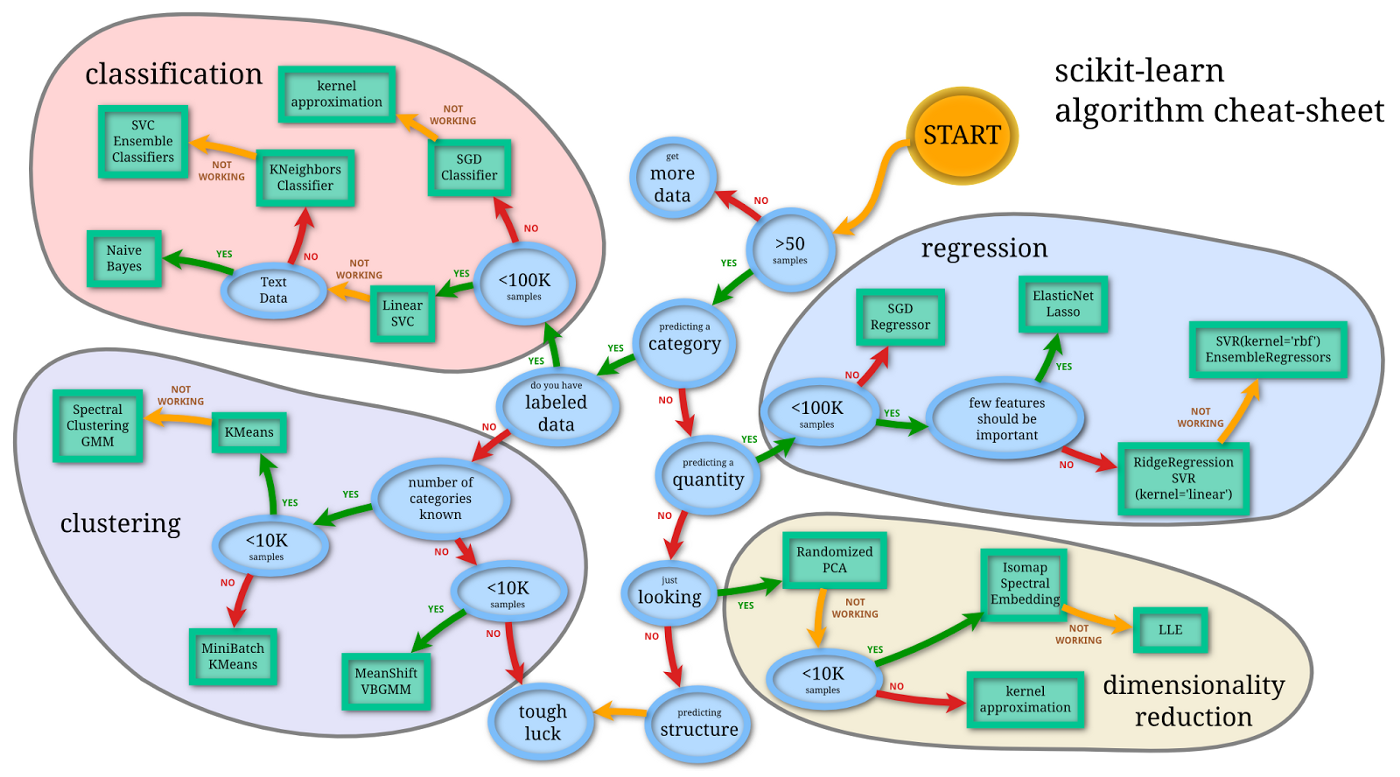
\includegraphics[height=0.8\textheight]{../figures/ml_cheatsheet.png}
\end{frame}

\begin{frame}{SVM for regression}
\begin{block}{Classification vs regression}
Classification: hyperplane separates different classes\\
Regression: hyperplane cluster the data sets
\end{block}
\end{frame}

\begin{frame}[fragile]
\frametitle{SVM usage}
\begin{block}{Model fitting example}
\begin{lstlisting}[language={python},frame=single]
from sklearn import svm
X = [[0, 0], [1, 1]]
y = [0, 1]
clf = svm.SVC(gamma='scale')
clf.fit(X, y)  
SVC(C=1.0, cache_size=200, class_weight=None, coef0=0.0,
    decision_function_shape='ovr', degree=3, gamma='scale', kernel='rbf',
    max_iter=-1, probability=False, random_state=None, shrinking=True,
    tol=0.001, verbose=False)
\end{lstlisting}
\end{block}
\begin{block}{Prediction of new value}
\begin{lstlisting}[language={python},frame=single]
clf.predict([[2., 2.]])
array([1])
\end{lstlisting}
\end{block}
\end{frame}

